\section{Architecture and Features}
\label{sec:arch}

PEBBL consists of two \emph{layers}, the \emph{serial layer} and the
\emph{parallel layer}.  The serial layer provides an object-oriented
means of describing branch-and-bound algorithms, with very little
reference to parallel implementation.  If you do not need parallelism,
or are simply in the early stages of algorithm development, the serial
layer allows branch-and-bound methods to be described, debugged, and
run in a familiar, serial programming environment.

The parallel layer contains the core code necessary to create parallel
versions of serial applications.  To parallelize a branch-and-bound
application developed with the serial layer, you simply define
new classes derived from \emph{both} the serial application and the parallel
layer.  A fully-operational parallel application only requires the
definition of a few additional methods for these derived classes,
principally to tell PEBBL how to pack application-specific problem and
subproblem data into MPI message buffers, and later unpack them.

Any parallel PEBBL application constructed in this way inherits the
full capabilities of the parallel layer, including a wide range of
different parallel work distribution and load balancing strategies,
and user-configurable levels of interprocessor communication.  You can
then add application-specific refinements to the parallelization, but
are not required to. Figure~\ref{fig:layers} shows the conceptual
relationship between the two layers, a serial application, and its
parallelization.  In the figure, the application is one of the
examples distributed with PEBBL, for solving binary knapsack problems;
the same basic pattern applies to all PEBBL applications.  The serial
layer class implementing the branch and bound algorithm is called
\texttt{binaryKnapsack}, and the parallel application is called
\texttt{parallelBinaryKnapsack}.  The ``diamond'' inheritance
structure shown in Figure~\ref{fig:layers} is integral to PEBBL's
design --- it is a powerful but sometimes problematic use of C++
multiple inheritance.

\begin{figure}[tpb]
\begin{center}
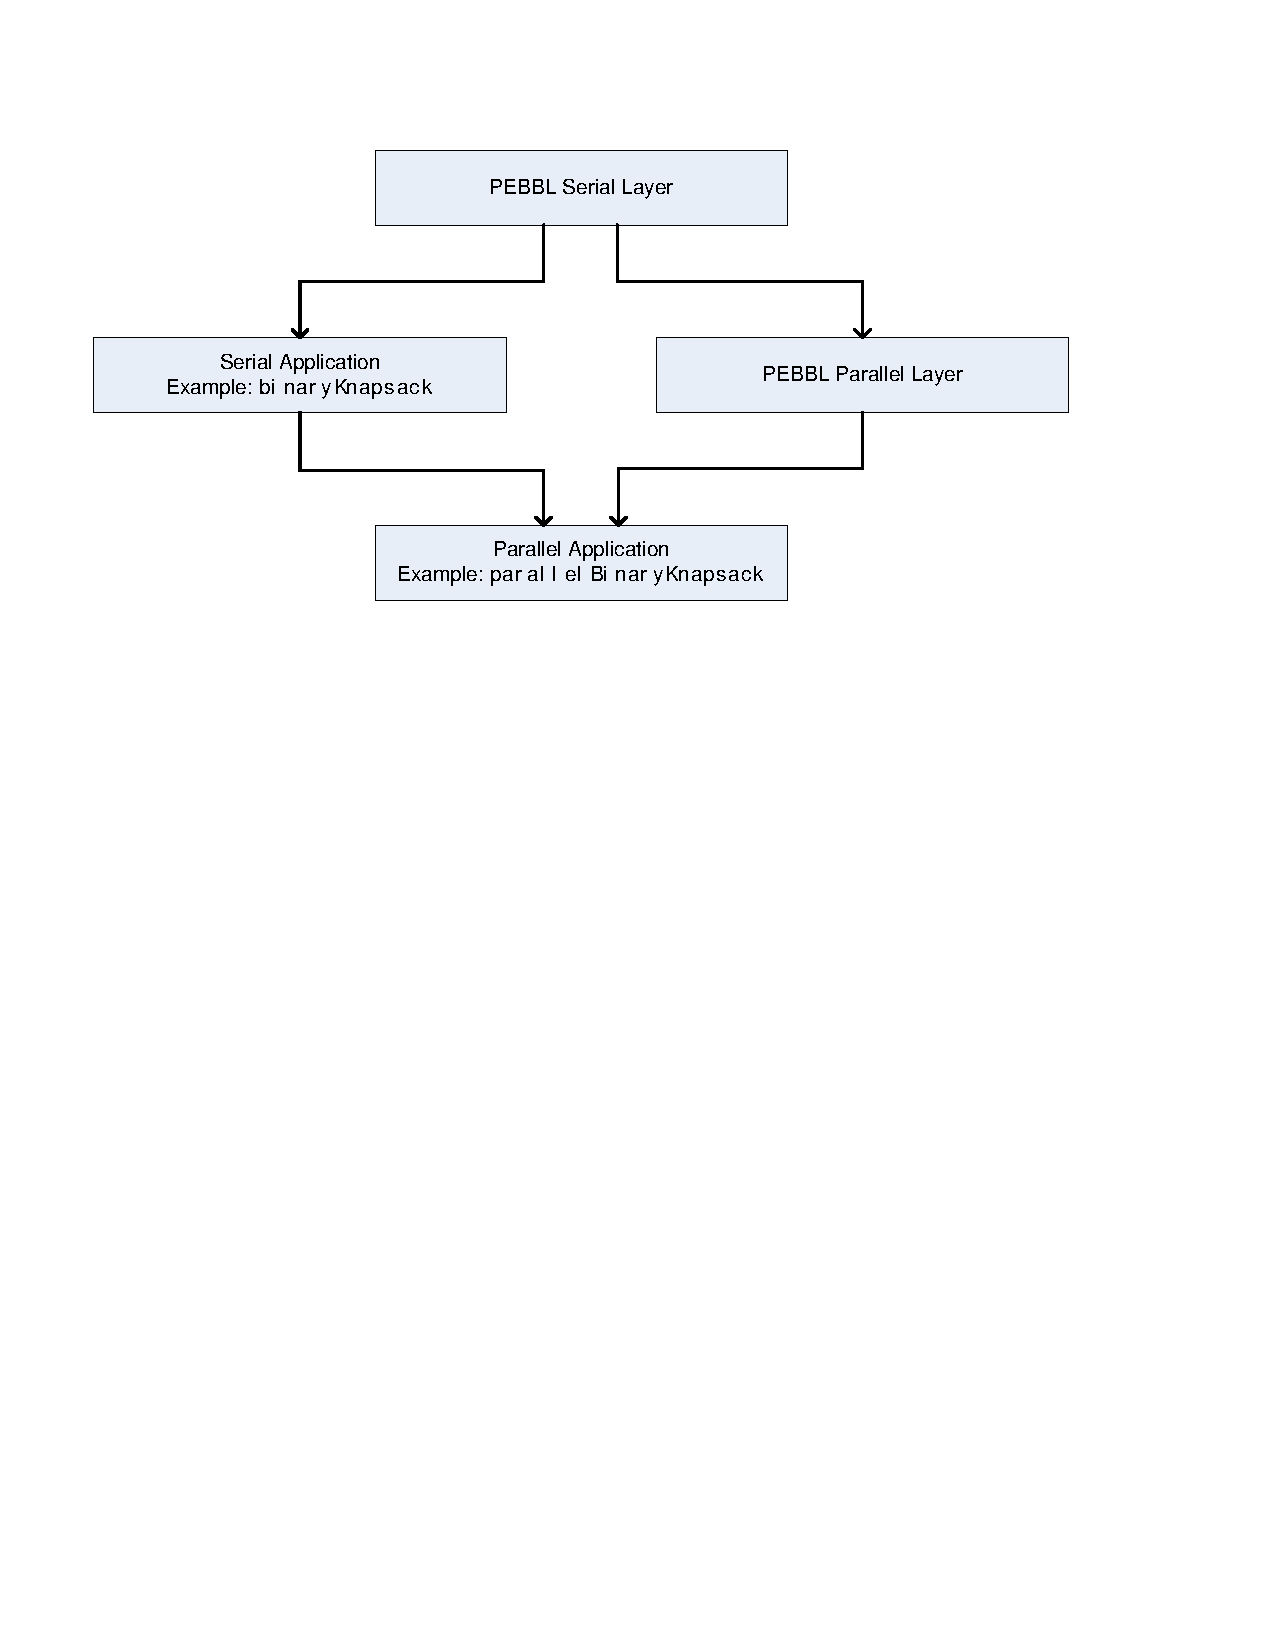
\includegraphics[width=\textwidth]{layers}
\vspace{-0.4in}
\end{center}
\caption{The conceptual relationships of PEBBL's serial layer, the
parallel layer, a serial application (in this case,
\texttt{binaryKnapsack}), and the corresponding parallel application
(in this case, \texttt{parallelBinaryKnapsack}).
\label{fig:layers}
}
\end{figure}


%% \subsection{The knapsack example}
%% This guide will use the binary knapsack problem as an example: given
%% $n$ items each with weight $w_i$ and value $v_i$, $i=1,\ldots,n$, find
%% a ``knapsack''or subset of items of maximum total value whose total
%% weight is less than some given value $C$.  Defining a variable $x_i$
%% to be $1$ if item $i$ is included in the subset, and $0$ otherwise,
%% this problem may be written
%% $$
%% \begin{array}{lll}
%% \max & \sum_{i=1}^n v_i x_i \\
%% \text{S.T.} & \sum_{i=1}^n w_i x_i \leq C \quad\quad \\
%% & x_i \in \{0,1\} & i=1,\ldots,n
%% \end{array}
%% $$ 
%% A simple upper bound on this problem may be computed as follows:
%% sort the items by decreasing $v_i/w_i$ and insert them into the
%% knapsack until no more will fit.  ADD MORE STUFF HERE.......


\subsection{Serial layer architecture}

\subsubsection{The \texttt{branching}, \texttt{branchSub}, 
               and \texttt{solution} classes}

To define a serial branch-and-bound algorithm, you must extend the two
or three key classes in the PEBBL serial layer, \texttt{branching},
\texttt{branchSub}, and possibly \texttt{solution}.  The
\texttt{branching} class stores global information about a problem
instance, and contains methods that implement various kinds of serial
branch-and-bound algorithms, as described below.  Each
\texttt{branchSub} object stores data about a subproblem (or node) in the
branch-and-bound tree, and the \texttt{branchSub} class contains
methods that perform generic operations on subproblems.  The
\texttt{solution} class stores a description of a feasible solution to
the problem.  PEBBL provides some standard \texttt{solution}-derived
template classes, essentially representing solutions as vectors of
standard C++ types such as \texttt{int} or \texttt{double}; for other
solution representations, users should create their own classes
derived from \texttt{solution}.  The basic
\texttt{branching}-\texttt{branchSub}-\texttt{solution} organization
of PEBBL is inspired by ABACUS~\cite{JT98}, but is more general, since
there is no assumption that cutting planes or linear programming are
involved.

By way of example of PEBBL's class structure,
our binary knapsack solver defines a class 
\texttt{binaryKnapsack}, derived from \texttt{branching}, to describe the
capacity of the knapsack and the possible items to be placed in it. We
also define a class \texttt{binKnapSub}, derived from
\texttt{branchSub}, which describes the status of the knapsack items
at nodes of the branching tree (\emph{i.e.}, included, excluded, or
undecided); this class describes a node of the branch-and-bound tree.
Each object in a subproblem class like \texttt{binKnapSub} contains a
pointer back to the corresponding instance of the ``global'' problem
class, in this case \texttt{binaryKnapsack}.  Through this pointer,
each subproblem object can find global information about the problem
instance and the overall
branch-and-bound process.  The knapsack application also defines a
class \texttt{binKnapSolution} derived from \texttt{solution}, to
represent solutions in a compact form that is particularly efficient
for large knapsack problems.

Both \texttt{branching} and
\texttt{branchSub} are derived from a common base class,
\texttt{pebblBase}, which mainly contains common symbol
definitions. The \texttt{branching} class also derives from
\texttt{pebblParams}, which holds command-line-specifiable
parameter objects implemented using the UTILIB class parameter
package.  The \texttt{solution} class also derives from
\texttt{pebblBase}.   Figure~\ref{fig:globalsub} illustrates the basic class
hierarchy for a serial PEBBL application.

\begin{figure}[tbp]
\begin{center}
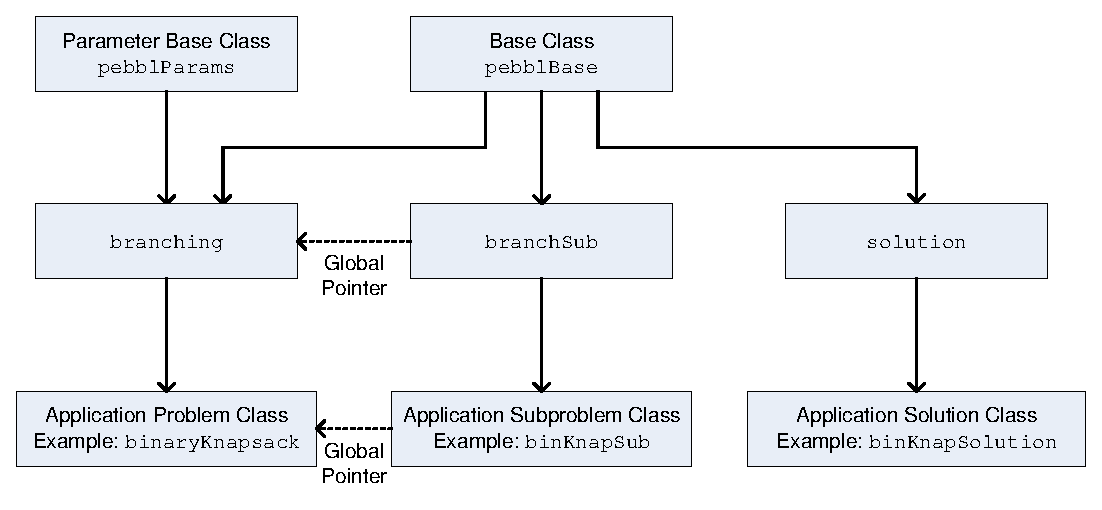
\includegraphics[width=\textwidth]{globalsub}
\vspace{-0.5in}
\end{center}
\caption{Basic class hierarcy for a serial PEBBL application (in this
case, 
\texttt{binaryKnapsack}, with corresponding subproblem class
\texttt{binKnapSub} and solution class \texttt{binKnapSolution}).}
\label{fig:globalsub}
\end{figure}

The class header file for the serial binary knapsack example is in
\url{acro-pebbl/packages/pebbl/src/example/pebbl/serialKnapsack.h}. Note that
\texttt{binaryKnapsack} is defined via
\begin{codeblock}
class binaryKnapsack : virtual public branching \{ $\cdots$ \}
$\;,$
\end{codeblock}
\texttt{binKnapSub} is defined via
\begin{codeblock}
class binKnapSub : virtual public branchSub $\cdots$ \{ $\cdots$ \}
$\;,$
\end{codeblock}
and \texttt{binKnapSolution} is defined via
\begin{codeblock}
class binKnapSolution : public solution $\cdots$ \{ $\cdots$ \} $\;.$
\end{codeblock}
In order for subsequent parallization to work properly, you should use
\texttt{virtual} when deriving classes from \texttt{branching} and
\texttt{branchSub}.  It is typically not necessary to use
\texttt{virtual} when deriving clases from \texttt{solution}.

Calculations made for subproblems frequently require data
stored in the problem description class, which are accessible via
pointers as depicted by the two horizontal dotted arrows in
Figure~\ref{fig:globalsub}.  To implement the upper arrow, the
definition of the subproblem class must instantiate the abstract
method \texttt{bGlobal()}; in \texttt{binKnapSub}, for example, this
capability is implemented via:
\begin{codeblock}
pro\=tected: \\
\>  binaryKnapsack* globalPtr;\\
public:\\
\>  inline binaryKnapsack* global() const \{ return globalPtr; \};\\
\>  branching* bGlobal() const \{ return global(); \};\\
\end{codeblock}
This pattern should be fairly typical: each object of the
\texttt{branchSub}-derived class should contain a pointer to the
\texttt{branching}-derived object for which it represents a
subproblem.  The \texttt{bGlobal()} method should then be implemented
by casting this pointer to a \texttt{branching*}.


\subsubsection{Manipulating subproblem states}
A key feature of PEBBL, first published in Eckstein et al.~\cite{EPH00}, is that
subproblems remember their \emph{state}.  Each subproblem progresses
through as many as six of these states, \texttt{boundable},
\texttt{beingBounded}, \texttt{bounded}, \texttt{beingSeparated}, 
\texttt{separated}, and \texttt{dead}, as illustrated in
Figure~\ref{fig:states}.

\begin{figure}[tbp]
\begin{center}
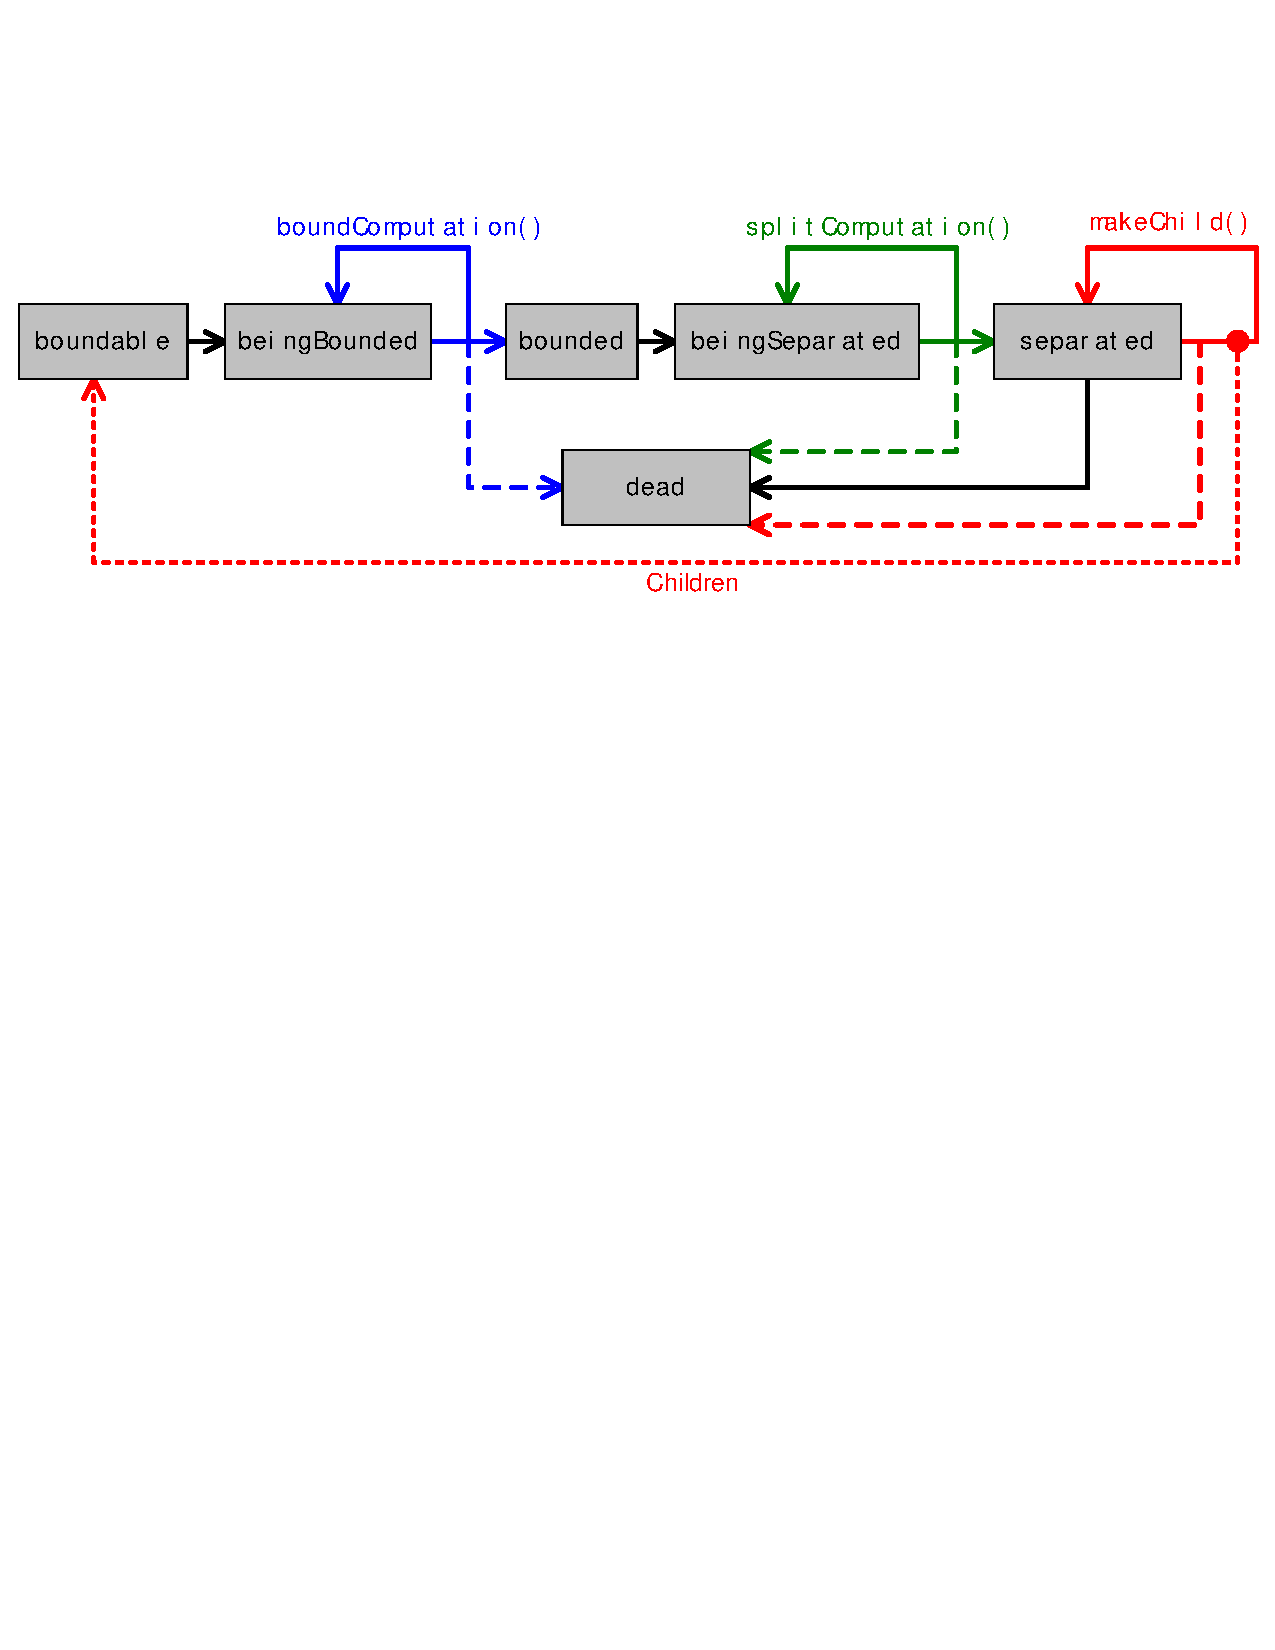
\includegraphics[width=\textwidth]{states-horizontal}
\vspace{-0.5in}
\end{center}
\caption{PEBBL's subproblem state transition diagram.  It is possible
that a single application of \texttt{boundComputation} may take a
subproblem from the \texttt{boundable} state, through
\texttt{beingBounded}, to \texttt{bounded}.  Similarly, a single use
of \texttt{splitComputation} may move a subproblem from
\texttt{bounded}, through \texttt{beingSeparated}, to
\texttt{separated}.}
\label{fig:states}
\end{figure}

A subproblem always comes into existence in state \texttt{boundable},
meaning that little or no bounding work has been done for it, although
it still has an associated bound value; typically, this bound value is
simply inherited from the parent subproblem.  Once PEBBL starts work on
bounding a subproblem, its state becomes \texttt{beingBounded}, and
when the bounding work is complete, the state becomes
\texttt{bounded}.

Once a problem is in the \texttt{bounded} state, PEBBL may elect to
split it into smaller subproblems.  At this point, the subproblem's
state becomes \texttt{beingSeparated}.  Once separation is complete,
the state becomes \texttt{separated}, at which point the subproblem's
children may be created.  Once the last child has been created, the
subproblem's state becomes \texttt{dead}, and it may be deleted from
memory.  Subproblems may also become \texttt{dead} at earlier points
in their existence, because they have been fathomed or represent
portions of the search space containing no feasible solutions.

Class \texttt{branchSub} has three key abstract virtual methods,
namely \texttt{boundComputation}, \texttt{splitComputation}, and
\texttt{makeChild}, that are responsible for applying these state
transitions to subproblems.  PEBBL's search framework interacts with
applications primarily through these methods; defining a PEBBL
branch-and-bound application essentially consists of providing
definitions for these three operators for the application subproblem
class ({\em e.g.} \texttt{binKnapSub}).

The \texttt{boundComputation} method's job is to move the subproblem
to the \texttt{bounded} state, updating the data member \texttt{bound}
to reflect the computed bound value.  The \texttt{boundComputation} method
is allowed to pause an indefinite number of times, leaving the
subproblem in the \texttt{beingBounded} state.  The only requirement
is that any subproblem will eventually become \texttt{bounded} after
some finite number of applications of \texttt{boundComputation}.  This
flexibility allows PEBBL to support branch-and-bound variants where 
bounding is suspended on a subproblem, the subproblem is set aside, and another
task or subproblem is considered.  The
subproblem's bound, reflected in the data member \texttt{bound}, may
change at each step of this process.  When \texttt{boundComputation}
decides that there is no more bounding work to be done for subproblem,
it should change the subproblem state to bounded by executing
\texttt{setState(bounded)}.  Changes in subproblem state should be
implemented via the \texttt{setState} rather than by direct assignment
to the data member \texttt{state} to ensure PEBBL can keep accurate
subproblem statistics.

The \texttt{splitComputation} method's job is similar to
\texttt{boundComputation}'s, but it manages the process of splitting
subproblems.  Eventually it must execute \texttt{setState(separated)}
to signal that the subproblem is completely separated, and then return
the number of child subproblems (\texttt{splitComputation} has a
return type of \texttt{int}).  Before that, however, it is allowed to
return an indefinite number of times with the problem left in the
\texttt{beingSeparated} state (in which case the return value is
ignored).  
This feature allows PEBBL to implement
branch-and-bound methods where the work in separating a subproblem is
substantial and might need to be paused to attend to some other
subproblem or task.  The subproblem's bound may be updated by
\texttt{splitComputation} if the separation process yields additional
bounding information.

Finally, \texttt{makeChild} returns a \texttt{branchSub*} pointing to
a single child of the subproblem it is applied to.  This parent must
be in the \texttt{separated} state.  After its last child has been
made, PEBBL automatically puts the subproblem in the \texttt{dead}
state.

If at any point in \texttt{boundComputation},
\texttt{splitComputation}, or \texttt{makeChild}, it becomes evident
that a subproblem does not require further investigation --- for
example, because it has become evident the subproblem is infeasible
--- one may mark the subproblem as \texttt{dead} by executing
\texttt{setState(dead)}.

In addition to \texttt{boundComputation}, \texttt{splitComputation},
and \texttt{makeChild}, some additional virtual methods must to be
defined to complete the specification of a branch-and-bound
application; all these methods are described in
Section~\ref{sec:serialMethods}.


\subsubsection{Pools, handlers, and the search framework}
\label{sec:framework}

PEBBL's serial layer orchestrates branch-and-bound search through a
module called the ``search framework'', literally,
\texttt{branching::searchFramework}.  The search framework acts as an
attachment point for two user-specifiable objects, a \emph{pool} and
a \emph{handler}, whose combination determines the exact ``flavor''
of branch and bound being implemented.

The pool object dictates how the currently active subproblems are
stored and accessed, which effectively determines the branch-and-bound
search order.  Currently, there are three kinds of pool: a heap sorted
by subproblem bound\footnote{Objects of type \texttt{branchSub} have a
member called \texttt{integralityMeasure} which may be used by the
application to measure how far a subproblem is from being completely
feasible (that is, from having \texttt{candidateSolution} yield
\texttt{true}; see Section~\ref{sec:serialMethods}).  If two
subproblems have identical bounds, the one with the lower
\texttt{integralityMeasure} will be placed higher in the heap, since
it presumably is more likely to lead to an improved incumbent
solution.}, a stack, and a FIFO queue.  If you specify the heap
pool, then PEBBL will follow a best-first search order; specifying the
stack pool results in a depth-first order, and specifying the queue
results in a breadth-first order. 

Critically, at any instant in time, the subproblems in the pool may in
principle represent any mix of states: for example, some might be
\texttt{boundable}, and others \texttt{separated}.  This feature gives
you flexibility in specifying the \emph{bounding protocol}, which is a
different aspect of the algorithm than the search order; each
``handler'' object implements a particular bounding protocol.

To illustrate what a bounding protocol is, consider the usual
branch-and-bound method for mixed integer programming as typically
described by operations researchers: one removes a subproblem from the
currently active pool, and computes its linear programming relaxation
bound.  If the bound is strong enough to fathom the subproblem, it is
discarded.  Otherwise, one selects a branching variable, creates two
child subproblems, and inserts them into the pool.  This type of
procedure is an example of what is often called ``lazy'' bounding (see
for instance~\cite{CP99}), because it views the bounding procedure as
something time-consuming (like solving a large linear program) that
should be delayed if possible.  In the PEBBL framework, lazy bounding
is implemented by a handler that tries to keep all subproblems in the
active pool in the \texttt{boundable} state.

An alternative approach, common in work originating from the computer
science community, is usually called ``eager'' bounding (again,
see~\cite{CP99} for an example of this terminology).  Here, all
subproblems in the pool have already been bounded.  One picks a
subproblem out of the pool, immediately separates it,
and then forms and bounds each of its children.  Children whose bounds do
not cause them to be fathomed are returned to the pool.  

Lazy and eager bounding each have their own advantages and
disadvantages, and the best choice may depend on both the application
and the implementation environment.  Typically, implementors seek to
postpone the most time-consuming operations in the hope that the
discovery of a better incumbent solution will make them unnecessary.
So, if the bounding operation is much more time-consuming than
separation, lazy bounding is most appealing.  If the bounding
operation is very quick, but separation more difficult, then eager
bounding would be more appropriate.  Eager bounding may save some
memory since leaf nodes of the search tree may be processed without
entering the pool, but has a larger task granularity, resulting in
lower parallel communication overhead per subproblem, but also
somewhat less potential for parallelism.

\begin{figure}[tbp]
\begin{center}
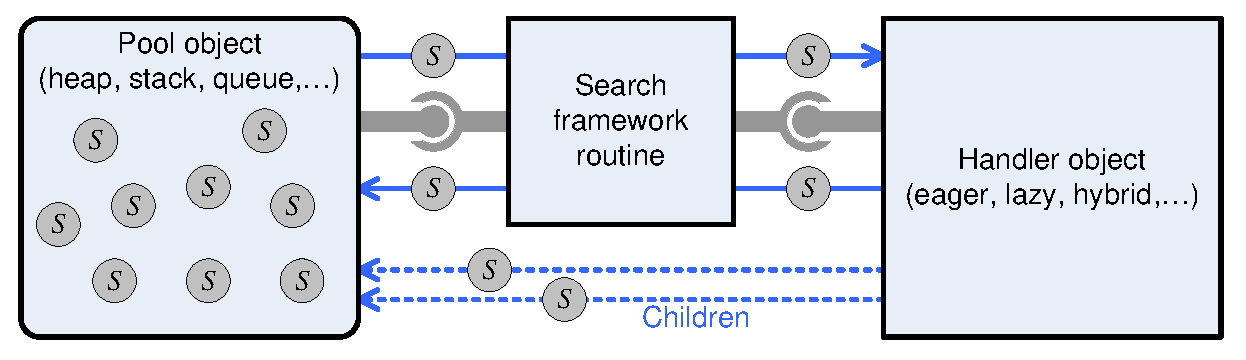
\includegraphics[width=\textwidth]{framework}
\vspace{-0.5in}
\end{center}
\caption{The search framework, pool, and handler.  Each $S$
indicates a branch-and-bound subproblem --- an object of type derived
from \texttt{branchSub}.}
\label{fig:poolandhandler}
\end{figure}

Because PEBBL's serial layer stores subproblem states and lets the
you specify a handler object, it gives you the freedom to specify
lazy bounding, eager bounding, or other protocols.  The search
framework routine simply extracts subproblems from the pool and passes
them to the handler until the pool becomes empty.  Currently, there
are three possible handlers, \texttt{eagerHandler},
\texttt{lazyHandler}, and \texttt{hybridHandler}.  The
\texttt{eagerHandler} and \texttt{lazyHandler} 
objects respectively implement eager
and lazy bounding by trying to keep as many subproblems
as possible in the \texttt{bounded} and \texttt{boundable} states,
respectively.

The \texttt{hybridHandler} object implements a strategy that is somewhere
between eager and lazy bounding, and is perhaps the most simple and
natural given PEBBL's concept of subproblem states.  Given any
subproblem, \texttt{hybridHandler} performs a single application of
either \texttt{boundComputation}, \texttt{splitComputation}, or
\texttt{makeChild}, to try to advance the subproblem one transition
through the state diagram of Figure~\ref{fig:states}.  
If the subproblem's state is
\texttt{boundable} or \texttt{beingBounded}, it applies
\texttt{boundComputation} once.  If the subproblem's state is
\texttt{bounded} or \texttt{beingSeparated}, it applies {\tt
splitComputation} once.  Finally, if the state is \texttt{separated},
the handler performs one call to \texttt{makeChild}, and inserts the
resulting subproblem into the pool.

The combination of multiple handlers, multiple pool implementations,
and the freedom in implementing \texttt{boundComputation} and
\texttt{splitComputation} create considerable flexibility in the kinds
of branch-and-bound methods that the serial layer can implement.
Figure~\ref{fig:poolandhandler} depicts the relationship of the search
framework, pool, and handler.

You may choose between the existing pools and handlers by setting
parameters in the \texttt{branching} class object; see
Section~\ref{sec:searchparams}.  You may also in principle supply
your own pools and handlers, but we consider that an advanced topic,
and it is not presently covered in this guide.


\subsection{Controlling the Search Process}

\subsubsection{Basic tolerances}

In its normal, non-enumeration 
mode of operation, PEBBL's optimality criteria are
controlled by two parameters, \texttt{absTolerance} and
\texttt{relTolerance}, with respective default values $0$ and
$10^{-7}$. PEBBL attempts to locate a single problem solution that is
either within an additive distance \texttt{absTolerance} or a relative
distance \texttt{relTolerance} of optimality, whichever turns out to
be less restrictive.  For example, setting \texttt{relTolerance} to
$0.05$ would specify a solution with 5\% of optimality.


\subsubsection{Multiple solutions: enumeration criteria
  and the solution repository}

PEBBL can also function in an enumeration mode in which it stores
multiple feasible solutions to a problem.  Enumeration mode is
activated if any of the four parameters \texttt{enumAbsTolerance},
\texttt{enumRelTolerance}, \texttt{enumCutoff} or
\texttt{enumCount} is set.  The meaning of these parameters is as
follows:
\begin{description}
\item[\texttt{enumAbsTolerance}:] Find all solutions whose objective
  value is within \texttt{enumAbsTolerance} of the best possible.  For
  example, setting $\text{\texttt{enumAbsTolerance}}=6$ indicates you
  want all solutions within $6$ units of optimal.
\item[\texttt{enumRelTolerance}:]  Find all solutions within a
  relative distance \texttt{enumRelTolerance} of the best possible.
  For example, setting $\text{\texttt{enumRelTolerance}}=0.10$ specifies
  that PEBBL should enumerate all solutions within $10$\% of optimal. 
\item[\texttt{enumCutoff}:]  Find all solutions with an objective
  value better than this value.  For a minimization problem, for
  example, setting $\text{\texttt{enumCutoff}}=0$ instructs PEBBL to
  find all solutions with a negative objective value.
\item[\texttt{enumCount}:]  Find the best \texttt{enumCount}
  solutions; for example setting $\text{\texttt{enumCount}}=10$
  requires PEBBL to find the $10$ best solutions.
\end{description}

If you set more than one of these parameters, PEBBL returns only
solutions simultaneously meeting all the specified criteria.  For
example, setting $\text{\texttt{enumRelTolerance}}=0.05$ and
$\text{\texttt{enumCount}}=200$ means that PEBBL should return only
those solutions that are among the $200$ best and are also within
$5$\% of optimal.

The enumeration mechanism keeps a repository of feasible solutions
represented as objects of type derived from the \texttt{solution}
class, maintained both as a hash table and heap in reverse order of
solution quality --- that is, the solution on the top of the heap has
the worst objective value.  The hash table representation, along with
hashing and comparison and methods of the \texttt{solution} class,
prevents duplicate solutions from entering the repository.  Discovery
of a new best incumbent solution can cause solutions to be removed
from the repository if either \texttt{enumAbsTolerance} or
\texttt{enumRelTolerance} is set.  If \texttt{enumCount} is set and
the repository already contains \texttt{enumCount} solutions, then
entry of a new solution into the repository causes the previously
worst solution in the repository to be removed.


\subsubsection{The \texttt{solution} class}
\label{sec:solclass}
PEBBL represents optimization problem solutions by objects derived
from the abstract class \texttt{solution}.  PEBBL provides a template
class, \texttt{arraySolution<\emph{T}>}, which represents solutions as a
one-dimensional array or vector of type \texttt{\emph{T}}.  This solution
representation should be adequate for many applications; if it is not
convenient or efficient for a given application, users may create
their own \texttt{solution}-derived classes.  It is even possible for
a single application to use several different solution
representations.

To properly maintain the hash table used to filter out duplication
solutions, PEBBL needs a hash function that may be applied to
solutions, and a means of comparing two solutions to see if they are
duplicates.  The normal means of hashing and comparison are through
the \emph{sequence representation} of solutions.  The
\texttt{solution} class contains abstract methods
\texttt{sequenceLength}, \texttt{sequenceData}, and
\texttt{sequenceReset} whose purpose is to convert a solution to
sequence of \texttt{double}s, in such a way that two solutions may be
considered duplicates if and only if invoking these methods results in identical
behavior.  If these methods are implemented, PEBBL automatically
supplies a hash function in the method \texttt{computeHashValue}, and
comparison operator for solutions is the method \texttt{duplicateOf}.

It is possible to dispense with the sequence representation methods;
in this case, however, the user must provide their own explicit
implementations of \texttt{computeHashValue} and
\texttt{duplicateOf}.  Even if a sequence representation is defined,
users might want to override either of these methods in the interest
of efficiency.


\subsubsection{Early output and checkpointing}

Some of the calculations for which PEBBL is intended may be extremely
long-running, and thus vulnerable to data loss if a system crashes
or a job's time allocation is exhausted.  PEBBL has two features
designed to mitigate such data loss.  The first, \emph{early output},
tries to ensure that if a PEBBL run is interrupted, you can recover
the best solution found so far.  You enable this feature by setting
the parameter \texttt{earlyOutputMinutes} to some positive value $m$.
Each time PEBBL finds a new incumbent solution (that is, a solution
better than all previously found ones) that exists for at least $m$
minutes, it writes it to disk so that it is available if
the process crashes. Early output is also useful if you wish to
voluntarily terminate a run and still have access to the best feasible
solution computed so far.  
This feature may be useful in early testing of an application for which you
may not yet know appropriate tolerance values.  For example, if you initiate
a run with a \texttt{relTolerance} of 5\%, but after considerable computation,
the optimality 
gap is still 10\%, you may decide you are satisfied with the 10\%
tolerance.

The second data loss mitigation feature is \emph{checkpointing}, which
imposes more overhead on PEBBL, but is more powerful.  Checkpointing is
currently available only for the parallel layer; it is not available
in applications built solely on the serial layer.  The key parameter
controlling checkpointing is \texttt{checkPointMinutes}.  If this
parameter has a positive value $m$, PEBBL writes its complete
internal state to disk approximately every $m$ minutes. Each processor
writes a separate file, and the checkpointing feature requires that
each processor have access to file I/O, but not necessarily in a
shared directory.

The computation can be restarted from the time of the checkpoint by
specifying either of the command-line parameters \texttt{restart} or
\texttt{reconfigure}.  Using \texttt{restart} is faster, but
\texttt{reconfigure} allows one to restart with a different parallel
configuration --- for example, a different total number of processors.
To use \texttt{reconfigure}, all checkpoint files must be in (or moved
to) the same directory.

Some MPI implementations provide their own checkpointing capabilities.
PEBBL's checkpointing feature is independent of any such capabilities
and does not require them.  

The early output mechanism and enumeration mechanisms are
currently independent.  When using enumeration, the early output mechanism
simply outputs the best incumbent.  Checkpointing, however, is fully
compatible with enumerating multiple solutions: each checkpoint will
save the entire state of the solution repository.



\subsection{Parallel layer architecture}

PEBBL's parallel layer attempts to accelerate the branch-and-bound
process by using multiple processors, and requires some form of the
MPI message passing interface.  PEBBL's parallel layer will run on
shared-memory (SMP) systems, but only by using MPI to emulate a
message passing environment.  

PEBBL's primary mode of parallelism, as is standard in parallel branch
and bound, is to explore different nodes of the search tree
simultaneously on different processors.  However, PEBBL has the
optional capability to use different modes of parallelism during the
early stages of the search; see Section~\ref{sec:rampup} below.

For the most part, parallel-layer search node processing is carried
out by the same \texttt{boundComputation}, \texttt{splitComputation},
and \texttt{makeChild} methods as in serial layer.  Thus, once you
have created these methods for your application, parallel execution
should be available with little additional development effort.


\subsubsection{Inheritance pattern}

The parallel layer's capabilities are embodied in the classes
\texttt{parallelBranching} and {\tt paral\-lel\-BranchSub}, which have the
same function as \texttt{branching} and \texttt{branchSub},
respectively, except that they perform parallel search of the
branch-and-bound tree.  Both are derived from a common base
class \texttt{parallelPebblBase}, whose function is similar to
\texttt{pebblBase}, containing mainly common symbol definitions.
The class \texttt{parallelBranching} also derives from
\texttt{parallelPebblParams}, which contains a large number of
parameters for controlling parallel search.  Furthermore, each of
\texttt{parallelBranching} and {\tt parallelBranchSub} is derived from
the corresponding class in the serial layer.

To turn a serial application into a parallel application, one must
define two new classes.  The first is derived from
\texttt{parallelBranching} and the serial application global class.
In the knapsack example, for instance, we defined a new class
\texttt{parallelBinaryKnapsack} which has both
\texttt{parallelBranching} and \texttt{binaryKnapsack} as
\texttt{virtual} base classes.  We call this class the \emph{global
parallel class}.  For each problem instance, the information in the
global parallel class is replicated once on every processor.

This basic inheritance pattern is repeated for
parallel subproblem objects.  In the knapsack case, we defined a
parallel subproblem class \texttt{parBinKnapSub} to have
\texttt{virtual} \texttt{public} base classes \texttt{binKnapSub} and
\texttt{parallelBranchSub}.  As with the serial subproblems, each
instance of \texttt{parBinKnapSub} has a
\texttt{parallelBinaryKnapsack} pointer that allows it to locate
global problem information.  Figure~\ref{fig:parinherit} depicts the
inheritance structure for the parallel knapsack application.  The
classes \texttt{solution} and \texttt{binKnapSolution} are omitted
from the figure since their relationship is unchanged from
Figure~\ref{fig:globalsub}, although a few additional \texttt{virtual}
methods in \texttt{solution} may need
to be implemented for parallel operation.

\begin{figure}[tb]
\begin{center}
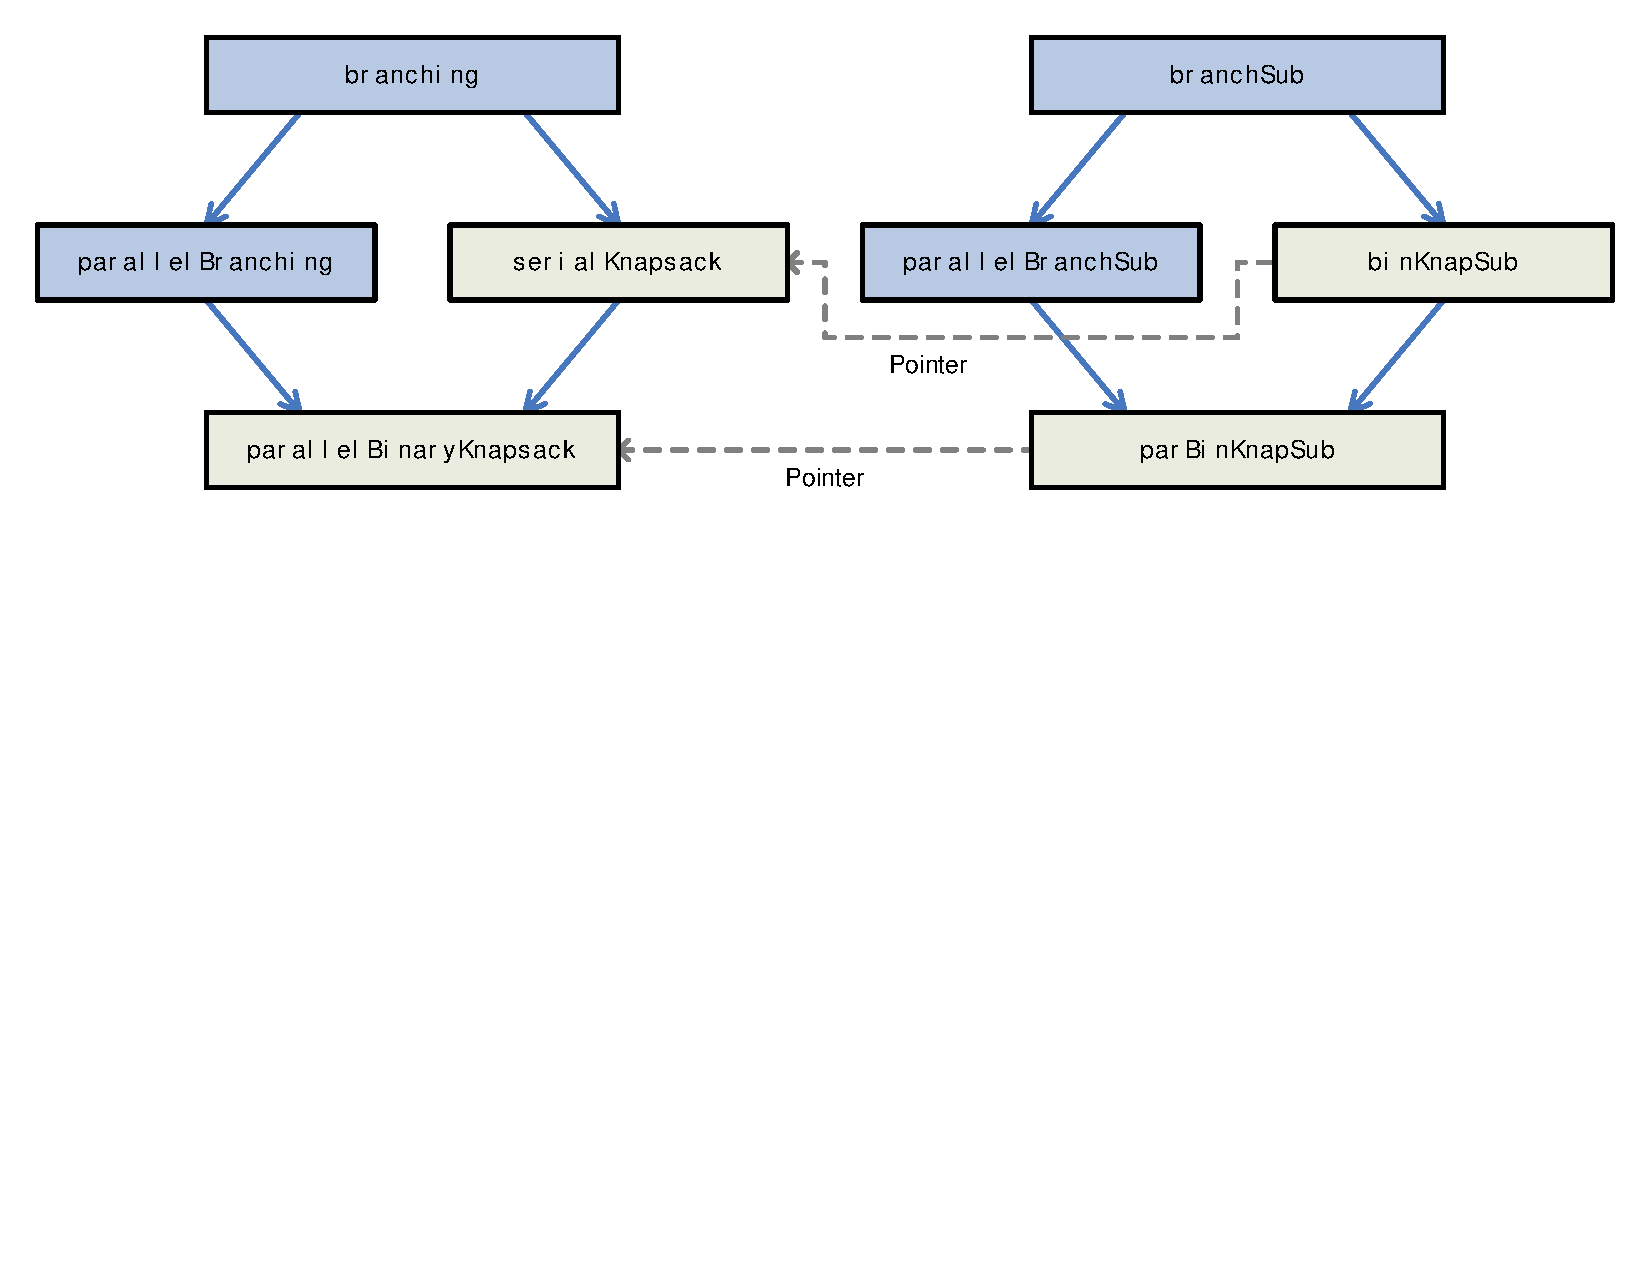
\includegraphics[width=\textwidth]{parinherit-new}
\vspace{-0.4in}
\end{center}
\caption{Partial depiction of the inheritance structure of the
  parallel knapsack application.  Other parallel applications are
  similar.}
\label{fig:parinherit}
\end{figure}

The header file
\url{acro-pebbl/packages/pebbl/src/example/pebbl/parKnapsack.h}
defines the inheritance structure depicted in
Figure~\ref{fig:parinherit}.  It defines
\texttt{parallelBinaryKnapsack} via
\begin{codeblock}
class \=parallelBinaryKnapsack : \\
\>public parallelBranching, \\
\>public binaryKnapsack \\
\{ \\
\>$\vdots$\\
\}$\;,$\\
\end{codeblock}
and \texttt{parBinKnapSub} via
\begin{codeblock}
cla\=ss \=parBinKnapSub : \\
\>\>public parallelBranchSub, \\
\>\>public binKnapSub \\
\{ \\
private: \\
\>parallelBinaryKnapsack* globalPtr; \\
public: \\
\>parallelBinaryKnapsack* global()  const \{ return globalPtr; \}; \\
\>parallelBranching*      pGlobal() const \{ return globalPtr; \}; \\
\>\>$\vdots$\\
\}
\end{codeblock}

Once this basic inheritance pattern is established, the parallel
application automatically combines the description of the application
coming from the serial application (in the knapsack case, embodied in
\texttt{binaryKnapsack} and \texttt{binKnapSub}) with the parallel
search capabilities of the the parallel layer.  For the parallel
application to function, however, additional methods must be defined,
as summarized in Section~\ref{sec:parMethods}.  The most critical of
these methods are \texttt{pack} and \texttt{unpack}, which must be
defined for the global parallel class, the subproblems, and solutions.
These methods respectively describe how to encode and decode objects
into a UTILIB \texttt{Packbuffer} or \texttt{UnPackBuffer}
object (see the UTILIB documentation).
%% For the global parallel class, PEBBL uses
%% \texttt{pack} and \texttt{unpack} when it broadcasts the problem
%% description to all processors at the outset of the parallel search.
%% For subproblems, PEBBL uses \texttt{pack} and \texttt{unpack} in the
%% transmission of subproblems between processors.

\subsubsection{Processor clustering}
\label{sec:clustering}
PEBBL's parallel layer employs a generalized form of the processor
organization used by the later versions of CMMIP~\cite{Eck94,Eck97}.
Processors are organized into \emph{clusters}, each with one
\emph{hub} processor and one or more \emph{worker} processors.  The
hub processor serves as a ``master'' in work-allocation decisions,
whereas the workers are in some sense ``slaves,'' doing the actual
work of bounding and separating subproblems. The degree of control
that the hub has over the workers may be varied by a number of
run-time parameters, and may not be as tight as a classic
``master-slave'' system.  Further, the hub processor has the option of
simultaneously functioning as a worker.

Three run-time parameters, all defined in \texttt{parallelPebblParams},
govern the partitioning of processors into clusters: {\tt
clusterSize}, \texttt{numClusters}, and \texttt{hubsDontWorkSize}.  First
PEBBL finds the size $k$ of a ``typical'' cluster via the formula
\begin{eqnarray*}
k &= &
\min \left\{ 
\mbox{\tt clusterSize},
\max \left\{
\left\lfloor \frac{\overline{p}}{\mbox{\tt numClusters}}
\right\rfloor,
1
\right\}
\right\} ,
\end{eqnarray*}
where $\overline{p}$ is the total number of processors.  Thus, $k$ is
the smaller of the cluster sizes that would be dictated by
\texttt{clusterSize} and \texttt{numClusters}.  Processors are then
gathered into clusters of size $k$, except that if $k$ does not evenly
divide $\overline{p}$, the last cluster will be of size
$\overline{p}\; \mbox{mod}\;k$.
In clusters whose size is greater than or equal to
\texttt{hubsDontWorkSize}, the hub processor is ``pure,'' that is, it
does not simultaneously function as a worker.  In clusters smaller
than \texttt{hubsDontWorkSize}, the hub processor is also a worker.
The rationale for this arrangement is that, in very small clusters,
the hub will be lightly loaded, and its spare CPU cycles should be
used to help explore the branch-and-bound tree.  If a cluster is too
big, however, using the hub simultaneously as a worker may
unacceptably delay the hub's response to messages, slowing down the
entire cluster.  In such cases, a ``pure'' hub is more advantageous.


\subsubsection{Tokens and work distribution within a cluster}
\label{sec:withincluster}
Unlike some ``master-slave'' implementations of branch and bound, each
PEBBL worker maintains its own pool of active subproblems.  This pool
may be any of the kinds of pools described in
Section~\ref{sec:framework}, although all workers must use the same pool
type.  Depending on various parameter settings, however,
the pool might be very small, in the most extreme case never holding more
than one subproblem.  Each worker processes its pool in the same
general manner as the serial layer: it picks subproblems out of the
pool and passes them to a search handler until the pool is empty.
When running in parallel, handlers have the additional ability to
\emph{release} subproblems from the worker to the hub.

For the remainder of this subsection, assume for simplicity that a
single cluster spans all available processors; in the next subsection,
we will amend our description to cover the case of multiple clusters.

\paragraph{Random release of subproblems:}
When running in a parallel context, \texttt{eagerHandler} decides
whether to release a subproblem as soon as it has become
\texttt{bounded}.  In parallel situations, \texttt{lazyHandler} and
\texttt{hybridHandler} make the release decision when they create a
subproblem.  The decision is a random one, with the probability of
release controlled by run-time parameters.  Released subproblems do
not return to the local pool; instead, the worker cedes control over
these subproblems to the hub.  Eventually, the hub may send control of
the subproblem back to the worker, or to another worker.

If the release probability is 100\%, then every subproblem is
released, and control of each subproblem is always returned to the hub at
a some point in its lifetime (at creation for \texttt{lazyHandler}
and \texttt{hybridHandler}, and upon reaching the \texttt{bounded} state
for \texttt{eagerHandler}).  In this case, the hub and its workers
function like a standard ``master-slave'' system.  When the
probability is lower, the hub and its workers are less tightly
coupled.  The release probability is controlled by the run-time
parameters \texttt{minScatterProb}, \texttt{targetScatterProb}, and
\texttt{maxScatterProb}.  The use of three different parameters,
instead of a single one, allows the release probability to be
sensitive to a worker's load.  Basically, if the worker appears to
have a fraction $1/w(c)$ of the total work in the cluster, $w(c)$
denotes the total number of workers in 
cluster $c$, then the worker uses the value \texttt{targetScatterProb}.
If it appears to have less work, then a smaller value is used, but no
smaller than \texttt{minScatterProb}; if it appears to have more work,
it uses a larger value, but no larger than \texttt{maxScatterProb}.

\paragraph{Subproblem tokens:}
When a subproblem is released, only a small portion of its data,
called a \emph{token}~\cite{RRM93,Eck94}, is actually sent to the hub.
The subproblem itself may move to a secondary pool, called the
\emph{server pool}, that resides on the worker.  A token consists of
only the information needed to identify a subproblem, locate it in the
server pool, and schedule it for execution.  Since the hub receives
only tokens from its workers, as opposed to entire subproblems, these
space savings translate into reduced storage requirements and
communication load at the hub.

When making tokens to represent new, \texttt{boundable} subproblems,
the parallel version of \texttt{lazyHandler} and \texttt{hybidHandler}
take an extra shortcut.  Instead of creating a new subproblem with
\texttt{parallelMakeChild} and then making a token that points to it,
they simply create a token pointing to the parent subproblem, with a
special field, \texttt{whichChild}, set to indicate that the token is
not for the subproblem itself, but for its children.  Optionally, a
single token can represent multiple children.  If every child of a
\texttt{separated} subproblem has been released, the subproblem is
moved from the worker pool to the server pool.

\paragraph{Hub operation and hub-worker interaction:}
Workers that are not simultaneously functioning as hubs periodically
send messages to their controlling hub processor.  These messages
contain blocks of released subproblem tokens, along with data about
the workload in the worker's subproblem pool, and other miscellaneous
status information.

The hub processor maintains a pool of subproblem tokens that it has
received from workers.  Again, this pool may be any one of the pools
described in Section~\ref{sec:framework}.  Each time it learns of a
change in workload status from one of its workers, the hub reevaluates
the work distribution in the cluster.  The hub tries to ensure that
each worker has a sufficient quantity of subproblems, and optionally,
that they are of sufficient quality (that is, with bounds sufficiently
far from the incumbent).  Quality balancing is controlled by the
boolean parameter \texttt{qualityBalance}, which is \texttt{true} by
default.  Workload quantity evaluation is via the parameter
\texttt{workerSPThreshHub}; if a worker appears to have fewer than
this many subproblems in its local pool, the hub judges it
``deserving'' of more subproblems.  If quality balancing is activated,
a worker is also judged deserving if the best bound in its pool is
worse than the best bound in the hub's pool by a factor exceeding the
parameter \texttt{qualityBalanceFactor}.  Of the workers that deserve
work, the hub designates the one with fewest subproblems as being most
deserving, unless this number exceeds \texttt{workerSPThreshHub}; in
that case, the workers are ranked in reverse order of the best
subproblem bound in their pools.

As long as there is a deserving worker and the hub's token pool is
nonempty, the hub picks a subproblem token from its pool and sends it
to the most deserving worker.  The message sending the subproblem may
not go directly to that worker, however; instead, it goes to the
worker that originally released the subproblem.  When that worker
receives the token, it forwards the necessary subproblem information
to the target worker, much as in~\cite{Eck94,Eck97,RRM93}.
This process will be described in more detail below.

When a single activation of the hub logic results in multiple
dispatch messages to be sent from the hub to the same worker, the hub
attempts to pack them, subject to an overall buffer length limit, into
a single MPI message, saving system overhead.

If the subproblem release probability is set to 100\%, and
\texttt{workerSPThreshHub} is set to $1$, the cluster will function
like a classic master-slave system.  The hub will control essentially
all the active subproblems, and send them to workers whenever those
workers become idle.  Less extreme parameter settings will reduce the
communication load substantially, however, at the cost of possibly
greater deviation from the search order that would have been followed
by a serial implementation.  Also, setting \texttt{workerSPThreshHub}
larger than $1$ helps to reduce worker idleness by giving each worker
a ``buffer'' of subproblems to keep it busy while messages are in
transit or the hub is attending to other workers.

The best setting of the parameters controlling the degree of
hub-worker communication depends on both the application and the
hardware, and may require some tuning, but the scheme has the advantage of
being highly flexible without any need for reimplementation or recompilation.

In addition to sending subproblems, the hub periodically broadcasts
overall workload information to its workers, so the workers know the
approximate relation of their own workloads to other workers' loads.  This
information allows each worker to adjust its probability of releasing
subproblems appropriately.

\paragraph{Rebalancing:}
If the probability of workers releasing their subproblems is set too
low, or the search process is nearing completion, 
workers in a cluster may have workloads that are
seriously out of balance, yet the hub's token pool may be empty.  In this
case, the hub has no work to send to underloaded workers.  To prevent
such difficulties, there is a secondary mechanism, called
``rebalancing,'' by which workers can send subproblem tokens to the
hub.  If a worker detects that it has a number of subproblems
exceeding a user-specifiable factor \texttt{workerMaxLoadFactor} times
the average load in the cluster, it selects a block of subproblems in
its local pool and releases them to the hub.  The hub can then
redistribute these subproblems to other workers.  

\subsubsection{Work distribution between clusters}
\label{sec:betweenclusters}
With any system-application combination, there will be a limit to the
cluster size that can operate efficiently, even if its hub does
not have any worker responsibilities.  To be able to use
all the available processors, it may then be necessary to partition
the system into multiple clusters.

PEBBL's method for distributing work between clusters resembles
CMMIP's~\cite{Eck94,Eck97}, with some additional generality: there are
two mechanisms for transferring work between clusters,
\emph{scattering} and \emph{load balancing}.  Scattering comes into
play when subproblems are released by workers.  If there are multiple
clusters, the worker makes a supplementary random decision as to
whether the subproblems should be released to the worker's own hub or
to a cluster chosen at random.  This random decision is controlled by
the apparent workload of the cluster relative to the entire system,
and the parameters \texttt{minNonLocalScatterProb},
\texttt{targetNonLocalScatterProb}, and
\texttt{maxNonLocalScatterProb}.  When choosing the cluster to scatter
to, the probability of picking any particular cluster is proportional
to the number of workers it contains (the worker's own cluster is
not excluded).

To supplement scattering, PEBBL also uses a form of ``rendezvous''
load balancing that resembles CMMIP's~\cite{Eck97};
\cite{MD93} and~\cite{KK92} also contain earlier, synchronous
applications of the same basic idea.  This procedure also has the
important side effect of gathering and distributing global information
on the amount of work in the system, which in turn facilitates control
of the scattering process, and is also critical to termination
detection in the multi-hub case.

Critical to the operation of the load balancing mechanism is the
concept of the \emph{workload} at a cluster $c$ at time $t$, which we
define as
\begin{eqnarray}
L(c,t) & = &\sum_{P \in C(c,t)} \!\!\!
{ \left| \overline{z}(c,t) - z(P,c,t) \right| }^{\rho}.
\label{loadcalc}
\end{eqnarray}
Here, $C(c,t)$ denotes the set of subproblems that $c$'s hub knows are
controlled by the cluster at time $t$, $\overline{z}(c,t)$ represents the
incumbent value known to cluster $c$'s hub at time $t$, and $z(P,c,t)$
is the best bound on the objective value of subproblem $P$ known to cluster
$c$'s hub at time $t$.  The exponent $\rho \in \{0, 1, 2, 3\}$
is set by the parameter \texttt{loadMeasureDegree}.  If $\rho=0$,
only the number of subproblems in the cluster matters.  Higher values of
$\rho$ give progressively higher ``weight'' to subproblems
farther from the incumbent.  The default value of $\rho$ is $1$.

PEBBL redistributes work between clusters using a ``rendezvous''
scheme that organizes all the cluster hub processors into a balanced
tree whose radix (branching factor) is determined by the parameter
\texttt{loadBalTreeRadix}, with a default value of $2$.  Periodically,
messages ``sweep'' through this entire tree, from the leaves to the
root, and then back down to the leaves.  For the details of the
rendezvous scheme, see~\cite[Section 4.4]{EPH00} or ~\cite[Section
4.3]{EPH00a}.  Peer-to-peer load balancing mechanisms are frequently
classified as either ``work stealing,'' that is, initiated by the
receiver, or ``work sharing,'' that is, initiated by the donor.  The
rendezvous method is neither; instead, donors and receivers
efficiently locate one another on an equal basis, possibly across a
large collection of processors.  Note that unlike ALPS~\cite{RLS04},
PEBBL does not employ a ``master of masters'' or ``hub of hubs''
processor, and its parallelization scheme is in principle indefinitely
scalable. 

The load balancing scheme has an important secondary function of
detecting termination, which can in general be challenging in highly
asynchronous parallel programs.  The general approach is a varient of
the ``four counters'' technique proposed in~\cite{Mat87}, although
only three counters are actually necessary.  More details may be found
in~\cite[Section 4.6]{EPH00} or ~\cite[Section 4.5]{EPH00a}.


\subsubsection{Ramp-up: starting the parallel search}
\label{sec:rampup}
\emph{Ramp-up} refers to the initial phase of a parallel search
algorithm when the number of active search nodes is of a smaller order
than the available processors.  In some branch-and-bound applications,
particularly when the number of processors is large, poor handling of
ramp-up can have significantly reduce parallel efficiency.

If only one processor at a time can work on a given search node, the
vast majority of processors will be idle during the initial
development of the search tree.  Often, this idleness is not a major
issue, because the search tree grows quickly.  However, in some
applications, the root node of the tree, and possibly nodes near
it, may take much longer to bound or separate than ``typical'' nodes
later in the search.  In such situations, the ramp-up phase is
elongated and it may be hard to make efficient use of all available
processors.

To help improve ramp-up performance, PEBBL implements
a special ramp-up phase in which the application may exploit
parallelism \emph{within} each subproblem, if it is available.  During
the ramp-up phase, all processors synchronously develop the same
search nodes around the root of the branch-and-bound tree.  During
this phase, the method \texttt{rampingUp()}, available in both
\texttt{parallelBranching} and \texttt{parallelBranchSub}, returns
\texttt{true}; otherwise, it returns \texttt{false}.  In response to
the value returned by \texttt{rampingUp()}, \texttt{boundComputation},
\texttt{splitComputation}, and even \texttt{makeChild} may then
attempt to explore some form of synchronous parallelism \emph{within} 
the processing of
individual search tree nodes.  These methods are free to conduct
MPI communication, but should be sure to leave all
processors in a uniform state upon exit.

Ramp-up execution is controlled by two virtual methods,
\texttt{continueRampup()} and
\texttt{force\linebreak[0]ContinueRampUp()}.  When both these methods
return \texttt{false}, PEBBL will terminate the ramp-up phase.  PEBBL
then automatically partitions the active search nodes, leaving each
worker processor with an approximately equal number of active
subproblems.  PEBBL then begins its standard, asynchronous
cluster/worker/hub search phase.

The default implementation of \texttt{continueRampup()} is controlled
by two parameters, \texttt{ramp\linebreak[0]UpPoolLimit} and
\texttt{rampUpPoolLimitFac}.  It returns \texttt{true} as long as the
number of active subproblems does not exceed $\max\{\mbox{\tt
rampUpPoolLimit}, \overline{p}\cdot\mbox{\tt rampUpPoolLimitFac}\}$,
where $\overline{p}$ is the total number of processors.  The default
implementation of \texttt{forceContinueRampUp()} is to return
\texttt{true} whenever the total number of subproblems created is does
not exceed the parameter \texttt{minRampUpSubprobsCreated}.  You may
override these rudimentary implementations with implementations more
specific to your application.


\subsubsection{Enumeration in parallel}

PEBBL's parallel layer now supports the same multiple-solution
enumeration criteria as its serial layer.  For scalability, storage of
the repository is partitioned approximately equally among all
processors through a mapping based on the solution hash value ---
every solution $s$ has a unique ``owning'' processor based on its hash
value.  Each processor has a local repository segment using the same
hash-table-and-heap representation as the serial layer's single
repository.

When enumeration is active and a solution $s$ is passed to
\texttt{foundSolution} on processor $p_0$, \texttt{foundSolution}
immediately uses $s$'s hash value to compute its owning processor
$p(s)$.  Unless $p(s)=p_0$, \texttt{foundSolution} immediately sends
the $s$ to processor $p(s)$.  Using the hash table representation of
the local portion of the repository and the \texttt{duplicateOf}
method, processor $p(s)$ then checks if $s$ is a duplicate of a
solution already in its local segment of the repository.  If so, it
simply discards $s$.  Otherwise, it enters $s$ into the local
repository.  At the end of the run, PEBBL uses a synchronous parallel
sort/merge algorithm to output a sorted list of all solutions found,
ordered from best objective value to worst.

Unless \texttt{enumCount} is in use, this logic is essentially all
that is needed.  If \texttt{enumCount} is set, however, the
implementation becomes more complicated.  In that case, for proper
pruning, PEBBL maintains an estimate of the
$\text{\texttt{enumCount}}^{\text{th}}$-best solution in the union of
the repository segments of all processors, which we call the
\emph{cutoff solution}.  To keep track of the cutoff solution, PEBBL
organizes all processors into a balanced tree.  By periodically
sending sorted arrays of solution values up this three, PEBBL computes
the current cutoff solution value, which it then broadcasts down the
tree.  This technique is not totally scalable with respect to the
value of \texttt{enumCount}, in that each processor potentially needs
sufficient storage to hold \texttt{enumCount} solution values and
identifier codes (but not entire solutions).


\subsubsection{On-processor multitasking: threads and the scheduler}

Once the ramp-up phase is over, the PEBBL parallel layer requires each
processor to perform a certain degree of multitasking.  PEBBL handles
the multitasking through what it calls ``threads'', although they are
not true threads, for example, in the POSIX sense: such true
multithreading would be incompatible with some MPI implementations and
MPP operating systems.  Instead, PEBBL uses \emph{non-preemptive}
threads, essentially coroutines that voluntarily and periodically
return control to a central scheduler module.

The PEBBL scheduler module recognizes two main types of threads:
\emph{message-triggered} and \emph{compute} threads.  Each
message-triggered thread effectively ``listens'' for MPI messages with
a specific tag value.  If the scheduler detects a complete received
message with the specified tag, it activates the thread to process the
message (which may involve sending messages to other processors).  The
thread then returns to a dormant state until the scheduler detects the
next message with its specified tag.

If there are no messages pending processing, the scheduler instead
tries to activate the compute threads.  Each compute thread has a
\emph{bias} which may be considered as a kind of priority.  Among all
compute threads that have declared themselves ``ready'', the scheduler
tries to allocate CPU resources in proportion to the threads'
bias values.  Threads can adjust their bias values over time.  

\begin{figure}[tbp]
\begin{center}
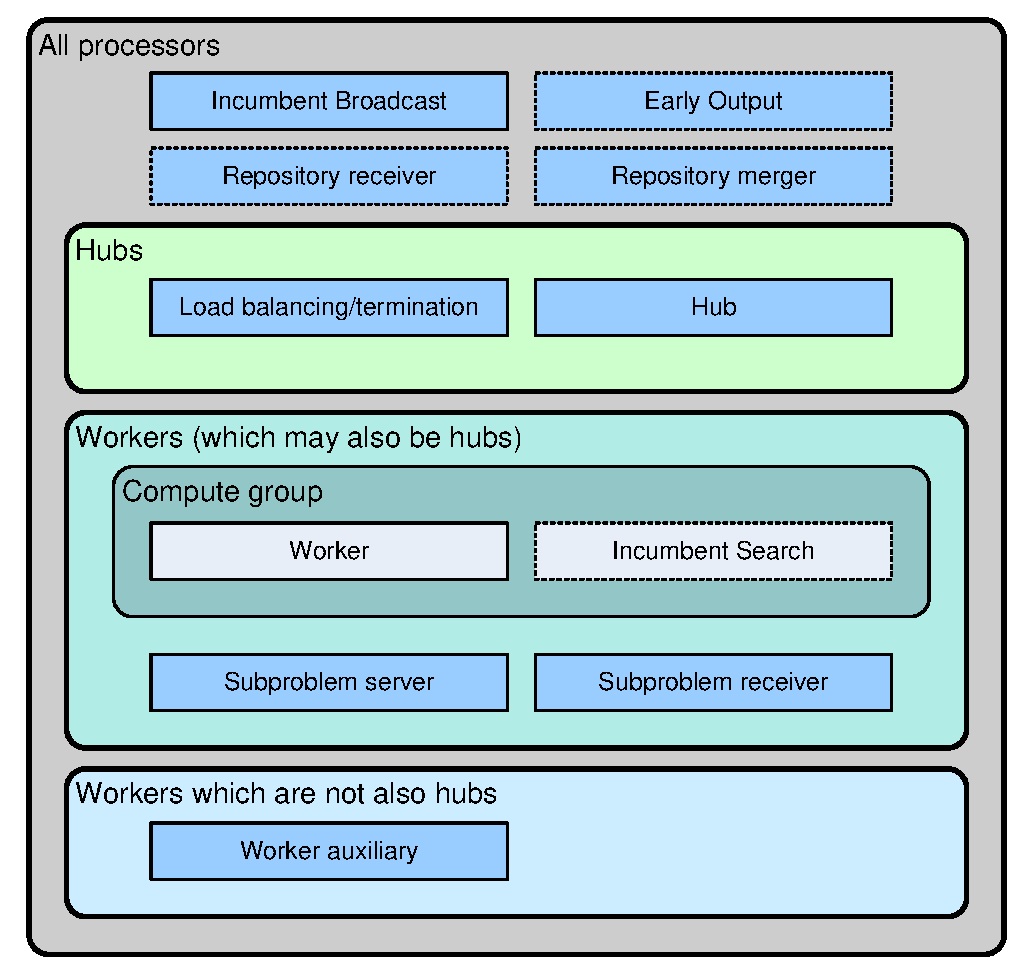
\includegraphics[width=0.7\textwidth]{threads-new}
\vspace{-0.2in}
\end{center}
\caption{PEBBL's standard threads.  A dashed outline
indicates that the thread may not exist in some cases.}
\label{fig:threads}
\end{figure}

Figure~\ref{fig:threads} depicts PEBBL's standard threads. You may add
additional threads of your own, but that is an advanced topic not
currently covered in this guide.  The standard threads are as follows:

\begin{description}

\item[Incumbent broadcast thread:] This message-triggered thread is
  active on all processors.  Its job is to make sure that all
  processors become aware, as soon as possible, of the objective value
  used to prune the search tree.  It implements a form of
  asynchronous broadcast using a tree with an adjustable branching
  factor.

\item[Early output thread:] This message-triggered thread is active on
  all processors if the parameter \texttt{earlyOutputMinutes} is
  positive; otherwise it is absent. This thread coordinates the
  process of writing solution files, making sure the file is written
  by a processor that is priviledged to do I/O (the MPI standard
  specifies that not all processors, and perhaps only one processor,
  must have file and console output capabilities).

\item[Repository receiver thread.]  This thread is active on all
  processors if PEBBL is enumerating multiple solutions.  It handles
  the receipt of most messages involved in coordinating the individual
  repository segments on each processor into a global asynchronous
  repository.

\item[Repository merger thread.]  This thread active is on all
  processors whenever the parameter \texttt{enumCount} is greater than
  1.  When \texttt{enumCount} is in use, certain messages required to
  maintain a global estimate of the cutoff solution may be sent on a
  time-delayed basis to limit peak message volumes; the repository
  merger thread handles this ``throttled'' message sending process.

\item[Hub thread:]  This thread is active on all hub processors, and
  responds to messages from workers; these messages contain
  acknowledgements of received subproblems, tokens for released
  subproblem, and worker load information.  Note that a hub
  processor's work distribution functions may also be activated in
  other situations besides receipt of one of these messages, via the
  \texttt{parallelBranching::activateHub()} method. 

\item[Load balancing/termination thread:] This thread is active on
  all hub processors, and manages termination detection.  It also
  controls checkpointing if \texttt{checkPointMinutes} is positive.  When
  there is more than one cluster, it also manages the balancing of
  workload between clusters.  It is generally message-triggered, but
  in multi-cluster situations it may also self-activate on some
  processors via the \texttt{ready()} predicate called by the scheduler.

\item[Worker thread:] This compute thread is active on all worker
  processors, and manages the processing of subproblems.

\item[Incumbent heuristic thread:] This optional compute thread may be
  active only on workers, and is controlled by the parameter
  \texttt{useIncumbentThread}.  Its purpose is to heuristically search
  for improved incumbent solutions.  Packaging this function into a
  compute thread allows PEBBL to directly control the fraction of CPU
  resources being dedicated to heuristic incumbent construction; the
  bias of this thread automatically adjusts based on the \emph{relative
  gap}, the relative difference between the incumbent value
  and the best known bound among active search tree nodes.  However,
  if the worker thread becomes idle (because it has no subproblems to
  process), the incumbent search thread will attempt to use all
  available CPU resources on the worker.  This behavior can be useful
  near the beginning of a run if the number of subproblems at the end of
  the ramp-up phase is less than the total number of worker
  processors: instead of being totally idle, worker
  processors attempt to heuristically find incumbents until their
  worker threads receive subproblems.

\item[Subproblem server thread:] This message-triggered thread is
  active on all worker processors.  It receives messages from the hub
  processors, and may in response send subproblems to other workers
  for processing.

\item[Subproblem receiver thread:]  This message-triggered thread is
  active on all worker processors, receiving subproblems for processing.

\item[Worker auxiliary thread:] This message-triggered thread is
  active on workers that are not also functioning as hubs.  The hubs
  send this thread various instructions, such as to write a
  checkpoint, check for termination, or terminate the search process.
  The worker auxiliary thread also periodially receives information
  relevant to the load balancing algorithms.

\end{description}

